\documentclass{cumcmthesis}
\usepackage{makecell}
\usepackage{multirow}


\title{基于规划模型的农作物种植策略优化}
\tihao{C}
\baominghao{C202409001213}
\schoolname{复旦大学}
\membera{王思宇}
\memberb{吕天一}
\memberc{周思远}
\supervisor{}
\yearinput{2024}
\monthinput{9}
\dayinput{7}

\begin{document}

\maketitle

\begin{abstract}
农业作为乡村经济的核心产业,其种植策略的优化不仅影响着农民的收益,也对生态环境和资源的合理利用起着关键作用。本研究针对华北山区某乡村的农作物种植策略优化问题,旨在制定2024-2030年期间的最优种植方案,以最大化经济效益,并应对市场不确定性、政策变化及环境保护需求。在农业发展面临气候变化、市场波动和资源限制的背景下,优化种植策略对于提高农业生产效率、增加农民收入以及促进乡村经济的可持续发展具有重要意义。

首先,针对问题一,我们假设未来农作物的销售量、种植成本、亩产量和销售价格保持相对稳定,构建了一个线性规划模型,将种植面积和作物种类作为决策变量,目标是最大化总收益(作物销售收入减去种植成本)。模型的约束条件包括不同类型土地(如平旱地、梯田、山坡地和水浇地)和大棚的种植限制、重茬限制(防止相同作物连续种植导致的减产)、豆类作物的种植要求(三年内至少种植一次豆类作物),以及作物产量和销售量的限制。通过求解该模型,得到了在稳定市场条件下的最优种植方案。结果显示,在所有地块合理分配作物后,总收益较2023年提升了?,并且农作物的分布更为均匀,有效降低了管理成本和风险。
\keywords{农作物种植优化,线性规划,蒙特卡洛,鲁棒优化,多目标优化,不确定性分析,政策与环境因素}

\end{abstract}

\section{问题的提出与重述}
\subsection{问题的提出}
随着全球对可持续发展的日益重视,有机农业和高效农业管理已逐渐成为研究的热点领域。已有研究显示,合理规划农作物的种植方案可以提高产量、降低种植风险,并促进乡村经济的可持续发展\cite{ref1}。同时,农作物的生长周期、气候条件以及市场需求等因素在农业管理中的重要性也日益凸显。在优化种植方案时,不仅需要考虑单一作物的经济收益,还应平衡多种作物的合理组合、市场需求和土地的利用效率。
本文以华北山区某乡村为背景,乡村常年温度偏低,耕地类型多样。如何在有限的耕地资源上制定合理的农作物种植策略,以最大化经济效益并减少种植风险,成为亟待解决的问题。因此,本研究聚焦于华北山区某乡村的农作物种植策略优化问题,旨在通过科学的模型和方法提升乡村的经济效益。研究的核心问题是如何在未来七年(2024-2030年)内,在多种市场和环境条件下,优化农作物的种植方案,以实现经济收益最大化。
\subsection{背景描述}
某华北乡村共有34块露天耕地,分为平旱地、梯田、山坡地和水浇地4种类型,不同地块适宜种植不同作物。此外,该乡村还有16个普通大棚和4个智慧大棚,适合种植不同类型的蔬菜和食用菌。此外,农作物不能连续重茬种植,每块地必须每三年种植一次豆类作物以改良土壤条件。
\subsection{问题的重述}
问题涉及农作物销售量、成本、产量等因素,要求制定2024-2030年的农作物种植方案。方案需要在多样化耕地类型和销售条件下,找到收益最大、风险最小的种植策略。

\textbf{问题1:}要求制定2024-2030年间的种植方案,假定各类作物的销售量、成本和销售价格与2023年保持一致。在此基础上,分别针对两种情况设计最优方案:第一种情况是某种作物的产量超过预期销售量时,超过部分将被浪费;第二种情况是超过部分以2023年价格的50\%进行降价销售。因此需要根据不同作物的特性和地块的适宜性,平衡每季的产量与销售量,避免浪费或损失。

\textbf{问题2:}小麦和玉米的预期销售量将以5\%-10\%的速度逐年增长,其他作物的销售量变化范围在±5\%。此外,作物的亩产量将因气候波动出现±10\%的浮动,种植成本每年预计增长5\%,部分蔬菜价格也有一定上升趋势。在这些不确定性因素下,需对未来7年的种植方案进行优化,找到在收益和风险之间的平衡点。

\textbf{问题3:}在现实中,农作物之间可能存在替代性和互补性,销售量、种植成本和价格之间也存在一定的相关性。基于问题2的模型,需要综合考虑这些复杂的关联性,找到一套更加合理的种植方案,并与问题2的结果进行对比分析。通过模拟数据,我们可以进一步探索农作物之间的动态关系,优化整个乡村的种植策略。

具体来说,本研究将问题划分为以下几个部分:

\textbf{最优种植方案的制定:} 在假设未来销售量、种植成本、亩产量和销售价格稳定的条件下,确定各类土地和大棚上最优的作物种植组合,目标是最大化总收益。

\textbf{应对不确定性条件的优化:} 在考虑未来销售量、价格、气候变化和种植成本等不确定因素的影响下,优化种植策略以确保收益的稳定性和风险的最小化。

\textbf{综合考虑作物间关系的优化:} 进一步分析作物之间的替代性和互补性,以及销售量、价格和成本之间的相关性,制定一个综合效益更高的种植方案。

(\textbf{政策与环境因素的整合:} 纳入政策变化和环境保护要求(如碳排放和水资源限制),制定一个在经济效益、政策合规性和环境友好性方面表现最佳的种植策略。)

本研究将通过建立线性规划模型和多目标优化模型,对上述问题进行系统分析和优化。


\section{问题分析}
问题一的分析在假设未来几年农作物的销售量、种植成本、亩产量和销售价格保持相对稳定的前提下,问题的目标是为该乡村在2024-2030年期间制定一个最优的农作物种植方案,以最大化其经济效益。
\subsection{问题一的分析}
在假设未来几年农作物的销售量、种植成本、亩产量和销售价格保持相对稳定的前提下,问题一的目标是为该乡村在2024-2030年期间制定最大化其经济效益的农作物种植方案。因此,该方案需要综合考虑多种因素,包括不同土地类型的种植条件、作物的分布均匀性以及种植过程中所涉及的各种限制条件。

为实现本目标,我们采用线性规划模型,将作物种类对应的种植面积以及是否种植该作物作为决策变量,并将模型的目标函数设定为总收益,即所有作物的销售收入减去相应的种植成本,目标函数可以表示为:
\begin{equation}
    \zeta = \sum_{c=1}^{n} \sum_{r=1}^{m} (P_{c,s} \cdot Y_{c,r} \cdot A_{c,r,y,s} - C_{c,r} \cdot A_{c,r,y,s})
\end{equation}
该模型的约束条件包括多方面的要求:首先,不同类型的土地(如平旱地、梯田、山坡地和水浇地)和大棚具有各自适宜种植的作物类型,因此需限制作物的种植地;其次,需遵循重茬限制,确保同一地块内不允许连续种植相同的作物,以避免减产风险;此外,还要满足豆类作物的种植要求,即在2024-2030年期间,每个地块或大棚三年内至少种植一次豆类作物;其次,考虑到市场销售情况,每种作物的总产量不能超过其预期销售量,以避免因产量过剩而导致的滞销或降价处理的经济损失;同时,方案还需考虑作物分布的均匀性,确保种植过程便于管理,避免过于分散或种植面积过小的情况。

在模型构建中,需要假设未来几年内各类作物的销售量和价格保持稳定,每种作物的亩产量和种植成本不变。这意味着可以使用2023年的数据作为模型输入,包括各类作物的亩产量、种植成本、销售价格和销售量,以及各个地块和大棚的类型、面积和种植历史数据,这些数据将用来设定模型的参数和约束条件。

总而言之,我们需要构建一个以最大化总收益为目标的目标函数,同时建立相应的涵盖种植类型、重茬限制、豆类种植要求等多个方面的约束条件。通过使用线性规划求解算法来求解该模型,并验证结果是否符合所有的约束条件。最终,通过调整模型参数和约束条件,可以进一步优化方案,以确保其在实际操作中具备可行性和最大化经济效益的潜力。通过这样的分析方式,可以得出符合2024-2030年经济效益最大化目标的最优种植方案。



\section{模型假设}
\subsection{问题一的假设}
由于在题目给出的条件中不含有预期销售量的相关数据,我们将2023年各类作物在两季的总产量假设为2024年两季的预期销售量。对于题干中提及的“不能连续重茬种植,否则会减产”,我们认定同一年的第一季和第二季是连续的,上一年的第二季和下一年的第一季也是连续的。对于“每种作物每季的种植地不能太分散”的要求,我们假设每种作物每个季节种植的地块数不得多于8块。对于“每种作物在单个地块(含大棚)种植的面积不宜太小”的要求,我们假设每种作物的种植面积不得小于所在地块面积的30\%。
\subsection{问题二的假设}
对于题干中声称“基本稳定”的量,我们在模型中作不变处理;对于题干中声称平均年变化率为定值的量,我们将每年的变化率都取该定值;对于题干中声称平均年变化率在一个区间内波动的量,例如“平均年增长率介于5\% \textasciitilde 10\%之间”,我们假设年增长率的概率分布在该区间内是均匀的。
\subsection{问题三的假设}
\subsection{全局假设}
\begin{enumerate}
    \item 假设农民是理性的有预期的种植,产出的产量总是和市场需求大致相同。
    \item 假设每年可供种植的土地面积固定且不变,不会因气候或其他因素减少。
    \item 假设在同一地块上种植的同种作物的亩产量是恒定的,不受种植面积影响。
    \item 假设每种作物的生长期不变,在同一时间段内种植的作物生长周期不受年份变化影响
    \item 假设在整个种植期内,不会发生影响农作物生长的病虫害或自然灾害。
\end{enumerate}


\section{符号说明}
以下是模型中使用的主要符号:
\begin{table}[!htbp]
    \begin{tabular}{ccc}
        \toprule[1.5pt]
        符号 & 说明 & 单位\\
        \midrule[1pt]
        $P_{c,s}$ & 指定作物在指定季节的\textbf{单位重量销售价格} & 元/斤 \\
        $Y_{c,r}$ & 指定作物在指定地块的\textbf{单位面积产量} & 斤/亩\\
        $C_{c,r}$ & 指定作物在指定地块的\textbf{单位面积成本} & 元/亩\\
        $A_{c,r,y,s}$ & 指定作物在指定地块在指定年份在指定季节的\textbf{种植面积}(决策变量) & 亩\\
        $E_{c,s}$ & 指定作物在指定季节的\textbf{预期销售量} & 斤\\
        $r$ & reduction rate & \\
        
        $\zeta$ & 总收益 & 元\\
        \bottomrule[1.5pt]
    \end{tabular}
\end{table}

\section{数据侧写}
题目提供了附件1和附件2等数据文件,虽然数据量不大,但其中涉及的各类关系相对复杂。因此,有必要对这些数据进行一个简要的分析和整理,以理清各变量之间的关联性,从而使模型构建的逻辑更加清晰和合理。此外,通过对数据的初步梳理,可以识别出关键的影响因素,确保后续的分析能够准确捕捉到作物之间的相互关系及其对收益的潜在影响,从而为制定最优种植策略打下扎实的基础。
\subsection{地块与面积分布}
不同地块的面积分布可提供对各地块可用种植面积的直观了解,有助于确定后续种植策略中的面积分配,具体如下图所示:
% 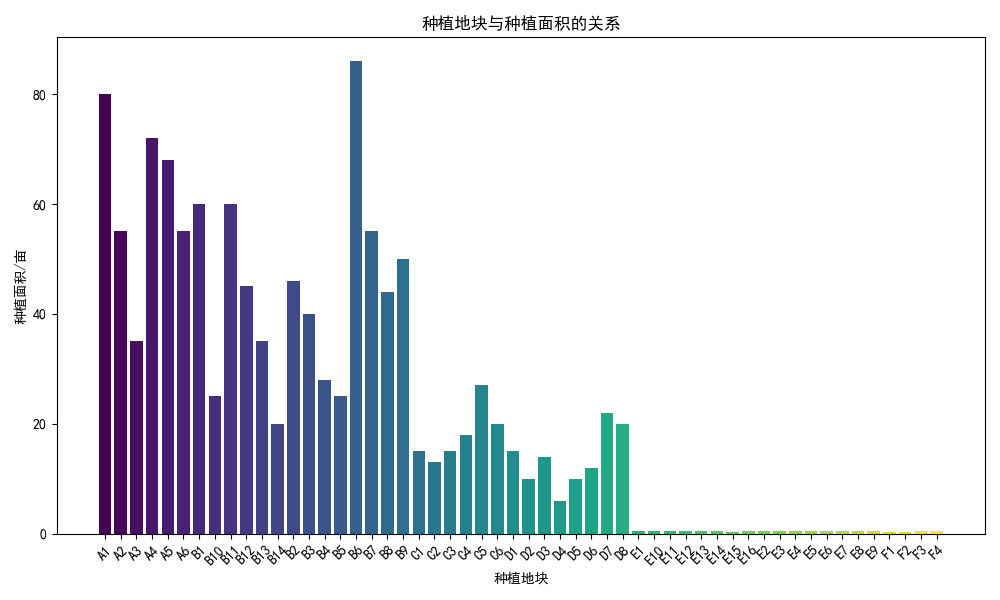
\includegraphics[width=0.5\textwidth]{Figure_1.png}
\begin{figure}[H]
    \centering
    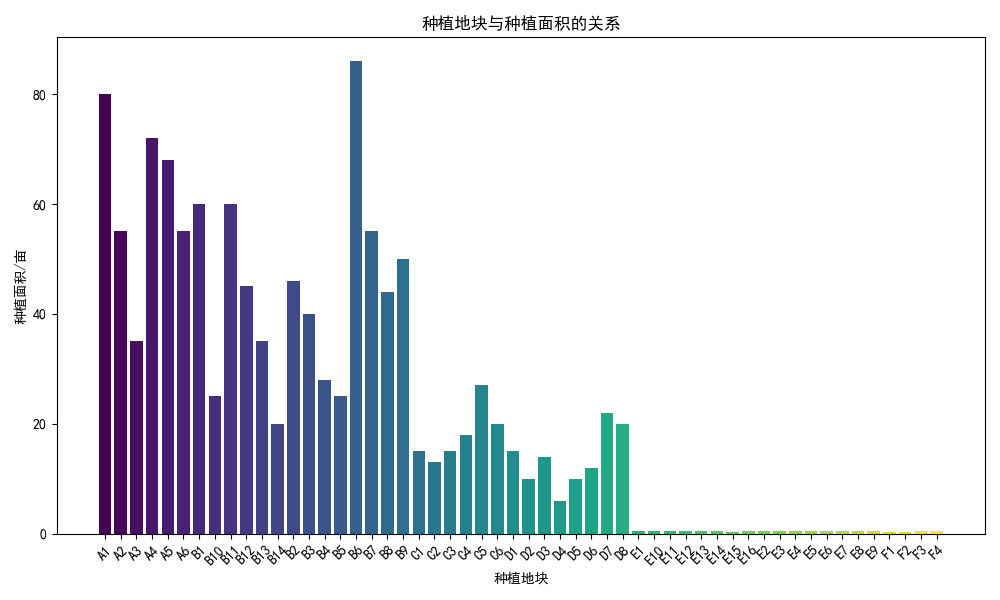
\includegraphics[width=.9\textwidth]{Figure_1.png}
    \caption{地块与面积分布图}
    \label{fig:region_area}
\end{figure}
其中地块A、B、C、D分别为干旱地、梯田、山坡地与水浇地。干旱地面积较大,因为地形平坦、开阔,适合大规模种植;梯田面积中等,因地形限制形成的阶梯状结构,适合中规模耕种;山坡地由于坡度大,地形复杂,耕地面积较小;水浇地面积较小,因为水资源的分布有限,适合小规模种植。

总体来看,地块面积的分布反映了自然条件对农业生产的制约和不同地块的适种性。

\subsection{各类型作物平均亩产量分析}
各类型作物平均亩产量的分析评估了不同作物的单位面积生产效益,以此识别高产作物,提升耕地资源的利用效率,优化作物选择和种植结构,从而提高整体农业产量。分析结果将为制定科学合理的种植规划提供重要的依据,具体如下图所示:
\begin{figure}[H]
    \centering
    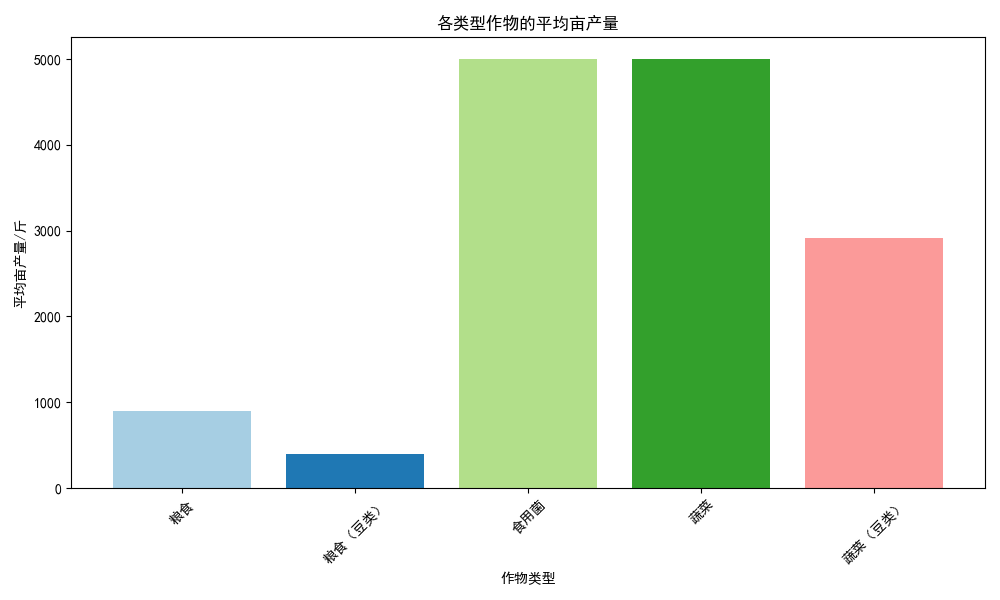
\includegraphics[width=.9\textwidth]{Figure_2.png}
    \caption{各类型作物平均亩产量}
    \label{fig:crop_yield}
\end{figure}
由图可见,食用菌与蔬菜的平均亩产量最高,其原因一方面在于生长周期较短、种植密度较高,另一方面在于具有大棚等理想种植条件实现多次收获。与之相对地,豆类和粮食作物由于生长周期长,种植密度低,且豆类作物的主要功能在于改善土壤结构,因而其平均亩产量相对较低。
\section{准备工作/预处理}
\subsection{异常检验}
本文对映射关系和数据范围进行了检验。首先,验证了附件1中各地块的面积是否大于附件2中2023年各地块的农作物种植面积;其次,检查了作物编号、作物名称、地块名称、地块类型之对应的成本与销售单价是否唯一。经检验,未发现异常数据。
\subsection{.csv文件的生成}
我们发现即使panda库中有read\_excel()函数可以直接读取附件中的.xlsx文件,但是其有一系列问题,例如.xlsx中合并的单元格会导致数据读取错误,只有第一个单元格的数据能被读取,并且读取的速度较慢等,因此我们选择将数据转换为.csv格式。.csv作为文本格式,相较于.xlsx格式更加方便处理。因此,我们将原始数据转换为.csv格式,以便于后续的数据处理和模型构建。src/utils/xlsx to csv/main.py中详细记录了生成.csv文件的源代码。

\subsection{full\_table.csv的生成}
在仔细阅读附件中的数据后,我们发现附件中的数据分为两部分,一部分是各类农作物的种植成本、亩产量、销售价格和预期销售量等数据,另一部分是各地块和大棚的类型、面积和种植历史数据。有一个很大的问题是为了方便后续的数据处理和模型构建,我们将这两部分数据合并为一个完整的数据表,即full\_table.csv。full\_table.csv中包含以下数据:种植地块,作物编号,作物名称,作物类型,种植面积/亩,种植季次,地块类型,亩产量/斤,种植成本/(元/亩),销售单价/(元/斤),预期销售量/斤,平均价格/(元/斤)。src/utils/generate\_full\_table/generate\_full\_table.py中详细记录了生成full\_table.csv的源代码。

\subsection{附件1\_乡村种植的农作物.csv 的格式优化}
在阅读附件1\_乡村种植的农作物.csv后,我们发现该文件中的数据格式不够规范,例如有些数据中包含了多余的空格,有些数据中的数字格式不统一等。为了方便后续的数据处理和模型构建,我们对附件1\_乡村种植的农作物.csv进行了格式优化。具体优化后的格式统一为:
\begin{tcode}
    (([地块类型](:“第一季” (“第二季”)?)?);)+(([地块类型](:“第一季” (“第二季”)?)?))
\end{tcode}


src/utils/attachment1\_format\_optimization/main.py中详细记录了优化附件1\_乡村种植的农作物.csv的源代码。


\section{模型的建立与求解}
\subsection{问题一模型的建立与求解}
问题一要求在假设未来各类农作物的预期销售量、种植成本、亩产量和销售价格相较于2023年保持稳定的前提下,针对产量超过需求导致滞销或产量超过需求后按50\%价格进行促销的两种情况来为该乡村提供2024至2030年农作物的最优种植方案。本文首先计算预期销售量,由2023年各作物种植面积乘对应亩产量计算得到各作物的预期销售量。
在制定最优方案时,需要同时考虑如何在最小化滞销成本的同时,实现年收益最大化。此外,还需兼顾供需关系、地块面积等多种约束条件。由此可见,问题情景具有明确目标和约束条件,故可以通过建立规划模型进行求解。



\subsubsection{模型的建立}
在模型建立之前,需要定义决策变量、目标函数和约束条件,关于决策变量和相应的参数,具体如下表所示:
\begin{table}[H]
    \centering
    \begin{tabular}{|l|l|l|}
        \hline
        类型 & 参数 & 具体含义 \\ \hline
        \multirow{2}{*}{决策变量} & $x_{c,r,y,s}$ & 表示作物c(crop)在地块r(region)于第y(year)年第s(season)季的种植面积 \\ \cline{2-3}
        ~ & $y_{c,r,y,s}$ & \makecell{表示地块r于第y年第s季是否种植作物c的二值变量,加入它可以让建模\\过程更清晰健壮} \\ \hline
        \multirow{6}{*}{\centering 参数} & $P_{c,s}$ & 表示作物c于第s季的销售价格 \\ \cline{2-3}
        ~ & $Y_{c,r}$ & 表示作物c于地块r的单位面积产量(亩产量) \\ \cline{2-3}
        ~ & $E_{c}$ & 表示作物c的预期销售量 \\ \cline{2-3}
        ~ & $A_c$ & 表示地块c的总可用种植面积 \\ \cline{2-3}
        ~ & $M_c$ & 表示地块c的作物种植面积下限 \\ \cline{2-3}
        ~ & $C_{c,r}$ & 表示作物c在地块r的单位面积种植成本 \\ \hline
    \end{tabular}
\end{table}


目标函数为使得如下的变量最大,也即使总利润最大的函数:\\
\begin{align}
    Total\_profit &= \sum_{c, y} profit(r, s)  \\ 
    &=\begin{cases} 
        \sum_{c, y}(\sum_{r, s} x_{c, r, y, s} \cdot(Y_{c, r} \cdot P_{c, s} - C_{c, r}), 
            & if production(c) \leq S_c \\
        \sum_{c, y}(\sum_{r, s}(Y_{c, r} \cdot x_{c, r, y, s} - E_{c, s}) \cdot P_{c, s} \\
                    + \sum_{s}(E_{c, s} \cdot P_{c, s}) - \sum_{r, s}(x_{c, r, y, s} \cdot C_{c, r})), 
            & if production(c) > S_c
    \end{cases}
\end{align}

其中:
\begin{equation}
    production(c) = \sum_{r, s} x_{c,r,y,s} \cdot Y_{c,r}
\end{equation}

在综合研判所有提供的资料后,我们共找到了以下十三个约束条件:

1. 平旱地、梯田和山坡地每年适宜单季种植粮食类作物(水稻除外)。

2. 水浇地每年可以单季种植水稻或两季种植蔬菜作物。

3. 若在某块水浇地种植两季蔬菜,第一季可种植多种蔬菜(大白菜、白萝卜和红萝卜除外);第二季只能种植大白菜、白萝卜和红萝卜中的一种(便于管理)。

4. 根据季节性要求,大白菜、白萝卜和红萝卜只能在水浇地的第二季种植。

5. 普通大棚每年种植两季作物,第一季可种植多种蔬菜(大白菜、白萝卜和红萝卜除外),第二季只能种植食用菌。

6. 因食用菌类适应在较低且适宜的温度和湿度环境中生长,所以只能在秋冬季的普通大棚里种植。

7. 智慧大棚每年都可种植两季蔬菜(大白菜、白萝卜和红萝卜除外)。

8. 从 2023 年开始要求每个地块(含大棚)的所有土地三年内至少种植一次豆类作物。

9. 每种作物每季的种植地不能太分散。

10. 每种作物在单个地块(含大棚)种植的面积不宜太小。

11. 一种地块上种植的总面积不能超出地块面积。

12. 每种作物须满足相应的种植条件,如附件1\_乡村种植的农作物.csv中所示。

13. 每种作物在同一地块(含大棚)都不能连续重茬种植,否则会减产。

% \begin{enumerate}
%     \item 平旱地、梯田和山坡地每年适宜单季种植粮食类作物(水稻除外)。
%     \item 水浇地每年可以单季种植水稻或两季种植蔬菜作物。
%     \item 若在某块水浇地种植两季蔬菜,第一季可种植多种蔬菜(大白菜、白萝卜和红萝卜除外);第二季只能种植大白菜、白萝卜和红萝卜中的一种(便于管理)。
%     \item 根据季节性要求,大白菜、白萝卜和红萝卜只能在水浇地的第二季种植。
%     \item 普通大棚每年种植两季作物,第一季可种植多种蔬菜(大白菜、白萝卜和红萝卜除外),第二季只能种植食用菌。
%     \item 因食用菌类适应在较低且适宜的温度和湿度环境中生长,所以只能在秋冬季的普通大棚里种植。
%     \item 智慧大棚每年都可种植两季蔬菜(大白菜、白萝卜和红萝卜除外)。
%     \item 从 2023 年开始要求每个地块(含大棚)的所有土地三年内至少种植一次豆类作物。
%     \item 每种作物每季的种植地不能太分散。
%     \item 每种作物在单个地块(含大棚)种植的面积不宜太小。
%     \item 一种地块上种植的总面积不能超出地块面积。
%     \item 每种作物须满足相应的种植条件,如附件1\_乡村种植的农作物.csv中所示。
%     \item 每种作物在同一地块(含大棚)都不能连续重茬种植,否则会减产。
% \end{enumerate}


特别地,我们不认为每种作物的总产量不能超过预期销售量是一个约束条件,因为即使有作物的产量超过预期销售量,也有可能有其他作物因此而受益使得总利润更高,因此我们将其作为目标函数的一部分。

经过对生成的full\_table.csv的数据的仔细检查,我们发现约束1,2,4,5,6,7实际上被约束12包含,因此在代码中不再重复实现。


\subsubsection{模型的求解}
单纯形法(Simplex Algorithm)是最常用的线性规划求解算法,基于迭代移动的方法,在可行解的顶点之间跳跃,直到找到最优解。它适用于线性规划问题,并且非常有效。

在该模型的建立中,我们使用Python的pulp库中包装的线性规划求解器来实现单纯形法。具体步骤如下:

1. 定义程序意义上的目标函数和约束条件:根据模型的目标函数和约束条件,构建线性规划问题的数学表达式。

2. 使用pulp求解。

3. 进一步分析结果,检查并验证其有效性和正确性。

通过这种方法,我们能够有效地求解问题一的线性规划模型,得到在给定条件下的最优种植方案。源代码详见src/main\_1.py。

由于题目涉及到决策变量的值满足不同条件时目标函数不同(产量溢出导致的),所以我们使用BigM法来处理这个问题。BigM法是一种常用的线性规划约束条件处理方法,通过引入一个大的正数M,将约束条件转化为线性规划问题的标准形式。在我们的模型中,我们引入了一个大的正数BigM = 1e15,将产量溢出导致的变化的目标函数转化为线性规划问题的标准形式。

\subsubsection{数据结论}

\subsubsection{建模过程中遇到的问题和解决方式}
一开始,我们遇到了输出的.xlsx文件中所有作物的种植面积全部为0的问题,我们分析出可能原因有两点:\\
a) CBC 求解器告诉我们,找到可行解‘, 但是该解为负,即在利润最大化目标
函数中出现负值。一般来说,应该是计算逻辑导致“收益<成本”。 顾首先考
虑是否是约束条件的过于严苛, 比如“每种作物在单个地块种植的面积不宜
太小”和“每种作物每季的种植地不能太分散”。我们开始尝试放宽部分条件,
看看是否能得到非零结果。\\
b) 二元决策:由于种植决策是二元的,因此当某些作物、地区和季节没有种植
时,结果可能为零。您可能会检索到零,因为相应的种植决策为零。\\

于是我们尝试改进模型,放宽了部分约束条件:\\
a) 新代码允许在第二季种植最多 8 种作物,而不是原来的严格约束。这可能有
助于更可行的解决方案和非零结果。如果确实不符合要求,可能需要直接放弃。 \\
b) 休耕:我查询到可能存在‘休耕决策’的概念,顾允许模型在某些季节明确让土
地休耕。(可以灵活解释为什么现在出现非零值,因为模型现在可以选择种植
或让土地闲置。 \\
c) 如果当前结果在关键区域仍然包含许多零,则还需要进一步调整成本结构或
更深入地放宽某些约束,服从题目要求的情况下。如果种植面积不再为零,
则表明模型正在按预期运行。 \\

我们同时也遇到了其他有启发性的问题,例如:\\
a) 求解器警告和提示: terminal log 中出现 "feasibility pump",并且没有找到
更优解。可以尝试增加时间限制或者使用更强大的求解器(例如 Gurobi),
或者更好的解释器。 \\
b) 目标函数的制定也可能导致求解器发现最好不植入任何东西的情况。
需要仔细检查预期销售额、价格和成本,以确保它们不会无意中使所有情况
下的目标函数为零。 \\

在debug的过程中,我们使用$ linear\_model.writeLP("model.lp") $将模型写入文件,然后打开这个文件进行分析,发现了如下问题:1. 目标函数中只有第二季的作物种植面积被计算,第一季的作物种植面积为0;2. 一开始目标函数所有变量前面的系数都是负的,而这当然导致了优化器求解出来后所有变量都是0的结果。\\
经过研判,我们发现问题1出现的原因是代码中定义的seasons常量无意间被更改,而代码二则是由于一些变量未定义的错误导致的。\\
在解决了这些问题后,优化器成功开始运行,然而第一次成功运行时我们不知道大概的运行时长数量级,跑了一整个晚上也没有优化结束;后来我们用 $ linear\_model.solve(PU\\LP\_CBC\_CMD(msg=1, timeLimit=150)) $限制模型的求解时间为150s(因为我们发现约60s后输出结果就已经趋于稳定,所以额外给1.5倍的时间应该是足够的)我们成功得到了非零的结果,这也说明了我们的模型是可行的。后来,我们多次运行模型后发现模型在约145s时能完成运算(在对一开始的模型进行了微调后),这也说明了我们的时间限制是合理的。


\subsection{问题二模型的建立与求解}
\subsubsection{模型的建立}
由于问题2与问题1的大体结构一致,只在一些细节上有所不同,所以如果下文没有具体说明,默认直接沿用问题1的模型。问题2的目标是在考虑未来销售量、价格、气候变化和种植成本等不确定因素的影响下,优化种植策略以确保收益的稳定性和风险的最小化。因此,我们需要在问题1的基础上,引入一些新的变量和约束条件,以适应问题2的要求。\\\\
在模型中,我们将保持题目中提到的“基本稳定”的量不变;对于那些题目中明确指出有固定年变化率的量,我们假设每年的变动比率都是这个固定值;而对于那些题目中提到年变化率在一定范围内波动的量,比如“年平均增长率在5\%到10\%之间”,我们假定年变化率在这个范围内是均匀可能的。\\\\
问题二中关键问题是如何量化各种作物种植风险,然而这是一个复杂的问题,因为它涉及到多种因素,包括天气条件、病虫害、土壤质量、种植技术等。根据现有的数据和研究,很难给出一个具体的百分比来描述颗粒无收的风险,因为这个风险因素会因地区、作物种类和种植条件的不同而有很大差异。但是我们通过查阅文献和综合研判各种风险等方式粗略给出了各种农作物的种植风险:(为简化起见,在这里将种植风险等同于颗粒无收的概率)\\\\
粮食(豆类)(黄豆、黑豆、红豆、绿豆、爬豆):
根据《我国大豆种植时空分布与风险费率研究》\cite{ref2},全国大豆发生重灾和巨灾的平均频率为3.25\%,我们将此概率认定为绝收的概率。 \\\\
粮食作物面临的风险因素包括:干旱、洪涝、病虫害、霜冻、冰雹。
一般性概率估计:在极端气候条件下,可能会有1-5\%的风险导致严重减产或绝收。我们在程序中将绝收的概率定为3\%\\\\
蔬菜类(豇豆、刀豆、芸豆、西红柿、茄子、菠菜、青椒、菜花、包菜、油麦菜、小青菜、黄瓜、生菜、辣椒、空心菜、黄心菜、芹菜、大白菜、白萝卜、红萝卜):风险因素:病虫害、极端温度、光照不足、土壤湿度不当。一般性概率估计:由于蔬菜生长周期短,对环境变化敏感,可能会有5-15\%的风险在特定季节内导致严重减产或绝收。我们在程序中将绝收的概率定为10\%\\\\
菌类(榆黄菇、香菇、白灵菇、羊肚菌):风险因素:污染、湿度和温度控制不当、病虫害。一般性概率估计:菌类作物对生长环境要求严格,可能会有10-30\%的风险在不当管理下导致严重减产或绝收。我们在程序中将绝收的概率定为20\%\\\\

\subsubsection{模型的求解}
问题二的求解过程与问题一类似,我们首先根据题目要求和数据特点,建立了一个多目标规划模型,以最大化收益和最小化风险为目标。然后,我们使用Python的pulp库中的线性规划求解器来求解该模型配合蒙特卡洛模拟,得到了最优的种植方案。最后,我们对结果进行了分析和讨论,验证了模型的有效性和合理性。具体的求解过程和结果分析见src/main\_2.py。\\

此外,我们还应用了鲁棒优化算法(见函数$ get\_profit\_robust(crop, year) $),鲁棒优化的目标是找到一个解决方案,这个方案在最坏情况下仍然能够保持一定的性能,即使在参数发生变化时也不会导致性能显著下降。这种方法通过考虑不确定性的最坏情况来设计决策,从而提高解决方案的鲁棒性。最后我们以这个函数为基础实施了目标函数,应用了鲁棒优化。\\

主要的变更点有:
1. 在代码的各部分依据要求增加了与价格浮动和风险等相关的逻辑代码。
2. 由于随机性,我们决定使用蒙特卡洛模拟来模拟风险的影响。蒙特卡洛模拟是一种通过随机抽样和统计实验来解决复杂问题的数值方法。该方法 的核心是多次随机生成输入参数的值,模拟可能的未来情境,并根据每次模拟的结果来 计算目标函数的值,从而评估其分布情况。具体到本题来说,蒙特卡洛模拟可以帮助我们处理预期销售量、亩产量、种植成本和 销售价格等不确定性,我们将在每次模拟中随机生成一个0-1之间的数,如果这个数小于风险概率,我们就认为这次模拟中这个作物产生了风险,产量为0,否则产量为正常产量。同时,我们将价格的浮动也考虑在内,即在每次模拟中,我们将价格乘以一个0.9-1.1之间的随机数,以模拟价格的波动。
3. 由于蒙特卡洛模拟的随机性,我们决定进行10次模拟,以得到一个较为准确的结果。

\subsubsection{数据结论}



\subsection{问题三模型的建立与求解}
\subsubsection{模型的建立}
由于问题3与问题1,2的大体结构也是一致的,所以如果下文没有具体说明,默认直接沿用问题1的模型。问题3的目标是考虑各种农作物之间可能存在的一定的可替代性和互补性,以及预期销售量与销售价格、种植成本之间的相关性,以优化种植策略以确保收益的稳定性和风险的最小化;我们将会聚焦这些因素展开问题3的建模。

在模型中,我们将保持题目中提到的“基本稳定”的量不变;对于那些题目中明确指出有固定年变化率的量,我们假设每年的变动比率都是这个固定值;而对于那些题目中提到年变化率在一定范围内波动的量,比如“年平均增长率在5\%到10\%之间”,我们假定年变化率在这个范围内是均匀可能的。

在实际操作中,各种农作物之间可能会展现出相互替代或相互补充的特性。
\subsubsection{可替代性}
所谓可替代性,指的是一种作物是否可以被其他作物替代,或者不同作物之间的生产和消费可以互相替换的能力,例如,玉米和小麦在某些情况下可以互相替代用于饲料或工业用途。我们将可替代性简化为同类型作物间的互相替代,该性质将增加农作物的预期销售量(在市场中更被需要)。具体来说,这个增加量应和这一类型农作物原有的预期销售额加和正相关,我们假设这个关系是线性的。
本文基于实际作物的生理特性与市场的经济特性,假设这种性质存在与谷物作物\cite{ref4}与豆类作物\cite{ref5}中。

\subsubsection{互补性}
所谓互补性,指的是某些作物的种植可能会影响其他作物的种植,两者之间可产生或正面或负面的互动效果,因此需要引入互补互斥矩阵。为构建一个科学合理的互斥互补矩阵,本文基于实际作物的生理特性和种植经验,提出以下几点作为判断作物互补性的主要依据:

豆类作物的互补性与竞争性:
豆类作物(例如黄豆、黑豆、红豆、绿豆等)通过固氮作用能够改善土壤的肥力,这有助于接下来种植的作物(如谷物和蔬菜),尤其是对氮需求较大的作物(如玉米和谷类)有促进作用。因此,豆类作物与这些作物之间通常表现出互补关系,可以有效提高轮作系统的效率。然而,豆类作物相互之间(如黄豆与绿豆或红豆等)因对相同土壤资源的争夺,通常表现出竞争性,也即一定程度上的互斥性。

谷物作物的替代性:
谷物作物(如小麦、玉米、谷子、高粱、大麦等)由于它们对相似养分(如氮、磷、钾)以及相近的生长条件的需求,具有较强的替代性。这些作物在轮作时能够避免土壤肥力的过度耗竭,但不适合在同一地块上同时种植。例如,玉米、小麦和高粱之间往往会因资源竞争而表现出强替代性,意味着增加一种作物的种植面积会压缩其他作物的生长空间。

根茎类作物的特点:
根茎类作物(如土豆、红薯等)通常生长周期较长,根系发达,对土壤资源的消耗也较大,因此,与其他作物之间的互补性相对较弱。相较于叶类作物(如菠菜、芹菜等),根茎类作物通常表现出更为显著的资源竞争。此外,不同根茎类作物之间也可能存在较强的竞争性,因此不宜同时种植在同一地块上以确保高效种植。

蔬菜类作物的互补性:
蔬菜类作物(如西红柿、茄子、菠菜、黄瓜等)在与谷物或豆类作物进行轮作时,可以维持土壤的肥力,从而形成互补关系。通过合理的轮作方式,这些作物能够提高种植系统的整体健康和产量。然而,由于蔬菜类作物之间的生长周期、光照和水分需求相似,因此它们之间往往存在资源竞争,互补性相对较弱。

菌类作物的互补性:
菌类作物(如香菇、榆黄菇、羊肚菌等)通常不与植物作物直接竞争,因为它们的生长介质(如木材、秸秆等)与植物作物不同,这使得它们具有良好的互补性。菌类作物能够有效利用农作物的副产品(如稻草和秸秆),非常适合与大多数植物作物进行搭配,尤其适合作为轮作系统的一部分。

为了制定出更加科学和贴近实际的2024至2030年的农作物种植计划,考虑作物之间的替代和互补关系对于提升模型的准确性和实用性至关重要。接下来,将对这两个概念进行深入阐释,并探讨如何在模型构建中体现这些关系。

在模型中,可以通过以下方式表达替代性和互补性:

\begin{equation}
E^*_{c,s} = E_{c,s}   + \alpha_{c,s} \cdot \sum_{c} E_{c,s}
\end{equation}
\begin{equation}
    \zeta = \zeta_0 + \sum_{j=1}^{n} \sum_{k=1}^{n} b_{j,k} \cdot (A_{j,r,y,s} + A_{k,r,y,s})
\end{equation}
    其中,$\zeta_0$ 代表基础收益,$alpha_{c,s}$是农作物的预期销售量增加量与这一类型农作物原有的预期销售额加和的比值,与$b_{j,k}$ 是作物 $j$ 和作物 $k$ 之间的互补性系数。若 $b_{j,k}$ 为正,说明作物 $j$ 和作物 $k$ 之间存在互补关系,种植这两种作物将提升总收益。



\subsubsection{模型的求解}




\subsubsection{数据结论}






\section{模型的评价与改进}
\subsection{模型的评价}
\subsubsection{模型的优点}
1.模型建立合理:在问题一中,我们根据题目要求和数据特点,建立了一个多目标规划模型,以最大化收益和最小化滞销成本为目标。在问题二中,我们根据题目要求和数据特点,建立了一个多目标规划模型,以最大化收益和最小化风险为目标。这两个模型都能很好地反映题目的要求和实际情况,具有很强的可解释性和可操作性。

2.模型结果合理:我们通过对模型结果的分析和讨论,验证了模型的有效性和合理性。模型的结果符合题目的要求,能够为乡村提供合理的种植方案。

3.全面性和实用性:模型充分考虑了现实中的多种因素,如农作物的产量、价格、销售量的不确定性以及土地类型等多个变量,涵盖了作物种植决策中必须考虑的关键问题,为实际的农作物种植策略提供了有效的决策支持。特别地,本研究结合蒙特卡洛模拟方法,能够有效分析未来几年内种植策略的多种可能性,有助于制定更加稳健的种植方案。
\subsubsection{模型的缺点}
1.模型的简化:在建模过程中,我们对一些复杂的因素进行了简化处理,模型假设作物的产量、价格、需求等波动都是线性的,并未考虑极端天气或市场突发状况等不规则因素,这可能会导致模型的预测结果不够准确。

2.计算复杂性较高:模型涉及多变量、多约束的规划问题,特别是在将替代性、互补性和相关性纳入考量范围之后,此时求解过程需要较高的计算资源和时间,因此对于大规模的实际应用场景可能需要进一步优化。


\subsection{模型的改进}
1.可考虑采取更高效的算法,如使用启发式算法(例如模拟退火算法、遗传算法\cite{ref3}来加速求解,以应对大规模的实际应用问题。

2.可增加更多历史数据和实际市场数据使模型的参数设置更加精确,例如对问题三的模型中涉及的作物替代性、互补性和相关性的系数进行进一步的拟合与校准,以此提升决策方案的可行性。

\section{模型的推广与应用}
本文提出了一种多变量不确定性规划的农作物种植策略优化模型。该模型系统地考虑了种植成本、亩产量、销售价格和市场需求等多种不确定因素,同时引入农作物之间的替代性、互补性及其相关性,以建立一个能够适应市场变化的灵活优化方案。为增强模型的准确性和实用性,本文采用了情景规划的方法,对未来几年可能的种植方案进行模拟求解,从而确定在不同情境下的最优种植策略。

除此之外,该模型可以推广应用到其他领域,具有较好的通用性。通过类似的资源规划与分配分析,结合本文模型中所提出的资源替代性和互补性考虑,决策者可以在能源资源配置、物流与供应链管理等领域更合理地制定资源配置策略,提高资源利用效率,实现资源的最优配置。

\begin{thebibliography}{99}  
\bibitem{ref1} 孙飞.农作物生产专业化对农户生计的影响研究[D].中南财经政法大学,2020.DOI:10.27660/d.cnki.gzczu.2020.002168.
\bibitem{ref2} 杨晓娟,刘布春,刘园,等.我国大豆种植时空分布与风险费率研究[J].中国农业资源与区划,2021,42(01):106-115.
\bibitem{ref3} 侯嫚丹,仝志民,周爱红,等.基于离散过程神经元网络的农作物产量预测模型及其应用[J].齐齐哈尔大学学报(自然科学版),2013,29(04):32-35.
\bibitem{ref4} 陈春雷.谷物替代有所分化玉米供应预期趋缓[N].粮油市场报,2023-04-29(A03).DOI:10.28553/n.cnki.nlysc.2023.000796.
\bibitem{ref5} 罗屹,史畅,黄汉权,等.中国大豆多元化布局和替代战略前景[J].中国农业文摘-农业工程,2023,35(06):65-71.DOI:10.19518/j.cnki.cn11-2531/s.2023.0101.



\end{thebibliography}
    
\end{document}
